\documentclass[12pt]{article}

\usepackage[utf8]{inputenc}
\usepackage[margin=1in]{geometry}
\renewcommand{\baselinestretch}{1}
\usepackage{indentfirst}

\usepackage{amsmath, amssymb}

\usepackage{hyperref}
\usepackage{cleveref}
\usepackage{graphicx}
\usepackage{float}
\graphicspath{{./figs/}}

\begin{document}

\begin{center}\begin{LARGE}
\textbf{Assignment 5: Results/Description}
\end{LARGE}\end{center}

\section*{Problem 1}

For this problem I have written two programs (\texttt{myFTCS} and
\texttt{myCN}) to solve the following problem. These may be compiled all
together with a \texttt{make all} as shown below.

\begin{figure}[H]
    \centering
    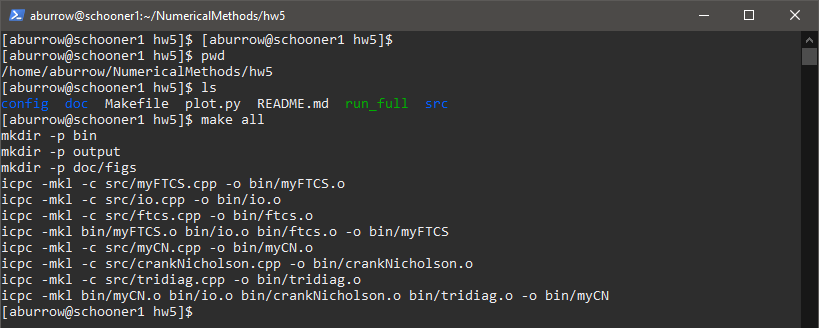
\includegraphics[width=1\textwidth]{compile}
    \label{fig:compile}
\end{figure}

This generates executables \texttt{myFTCS} and \texttt{myCN} in the ``./bin''
directory, which may be run one at a time. There is also a \texttt{plot.py} in
the root which may be run to generate plots from the output of the executables.
However, to run all these programs at once, I have also included a
\texttt{run\_full} bash script that may be executed for convenience.

In this problem, I use (a) the FTCS method and (b) the Crank-Nicholson method
to solve the diffusion equation
$$
\begin{aligned}
\frac{\partial n}{\partial t}
&= \frac{\partial^2 n}{\partial x^2}.
\end{aligned}
$$

\subsection*{(a)}

Below I run the program that demonstrates solving our differential equation
using the FTCS method:
\begin{figure}[H]
    \centering
    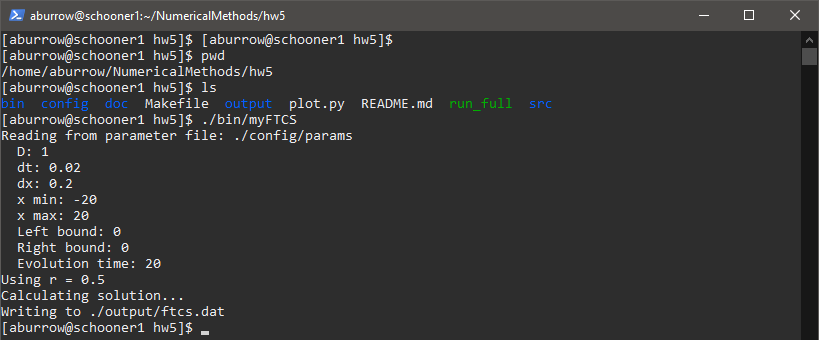
\includegraphics[width=1\textwidth]{myFTCS}
    \label{fig:myFTCS}
\end{figure}

\begin{figure}[ht]
    \centering
    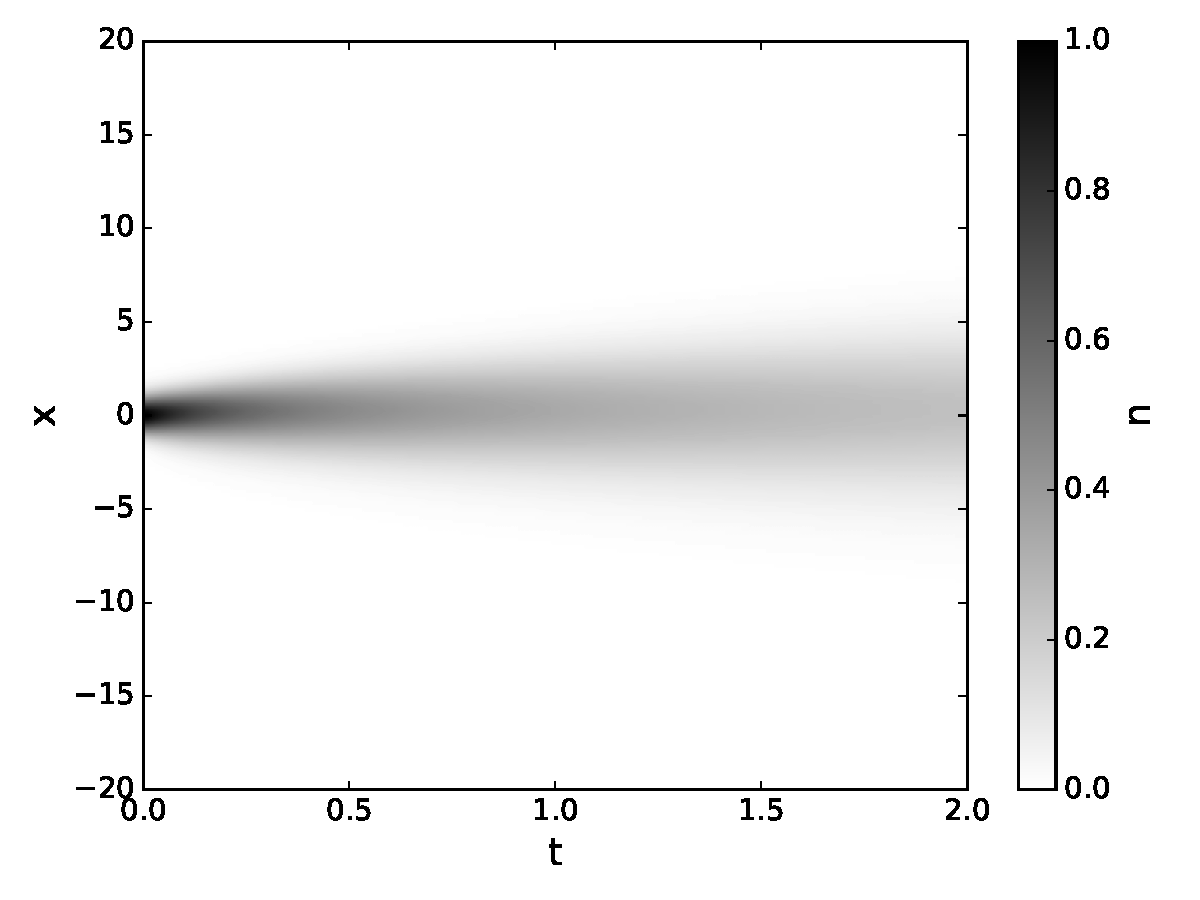
\includegraphics[width=0.9\textwidth]{ftcs}
    \caption{Solution using the FTCS method.}
    \label{fig:ftcs}
\end{figure}


\subsection*{(b)}

Below I run the program that demonstrates solving our differential equation
using the Crank-Nicholson method:
\begin{figure}[H]
    \centering
    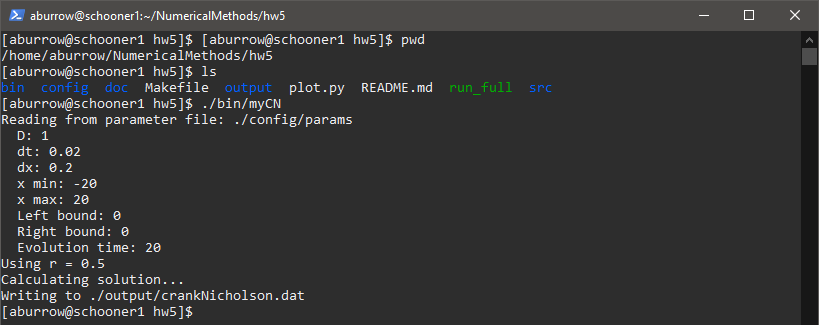
\includegraphics[width=1\textwidth]{myCN}
    \label{fig:myCN}
\end{figure}

\begin{figure}[ht]
    \centering
    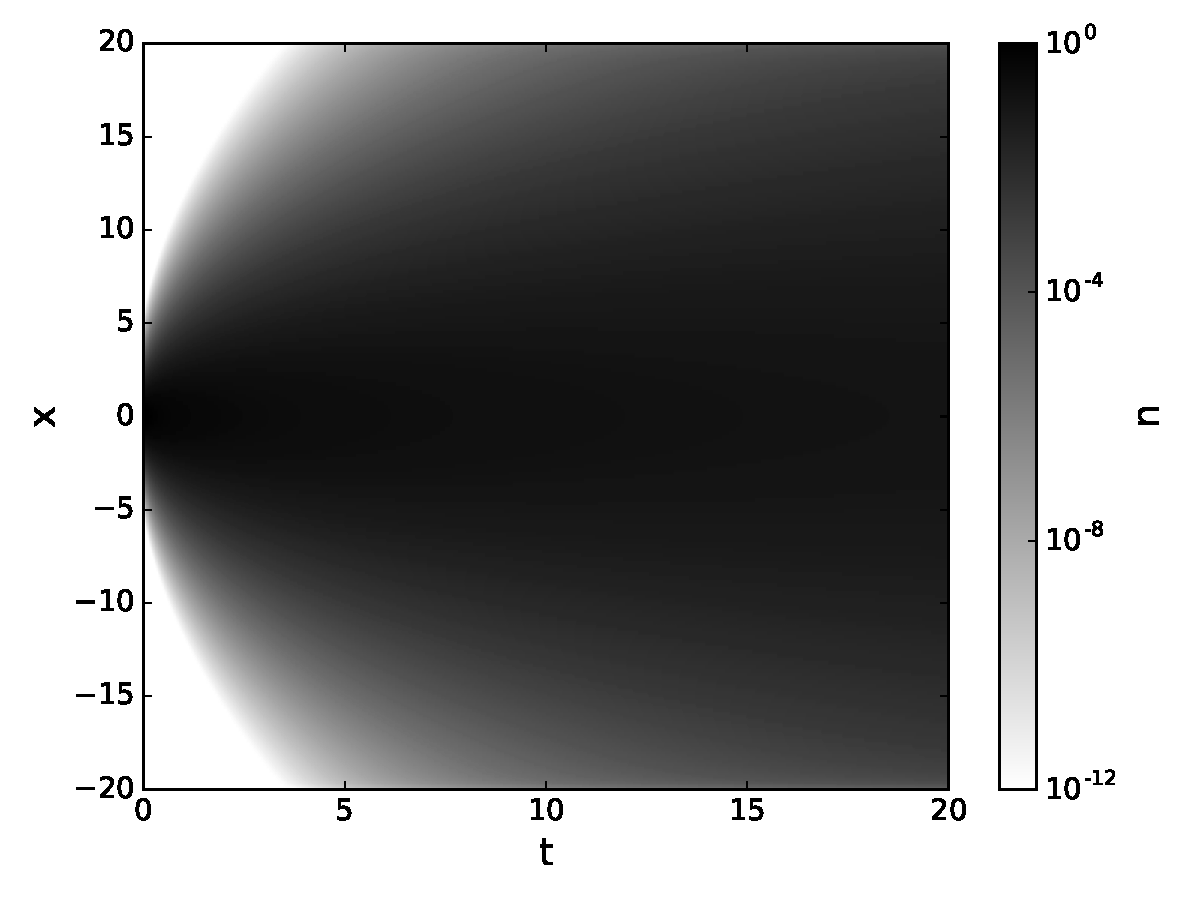
\includegraphics[width=0.9\textwidth]{crankNicholson}
    \caption{Solution using the Crank-Nicholson method.}
    \label{fig:crankNicholson}
\end{figure}


\end{document}
